\section{Phương pháp thu thập và lưu trữ dữ liệu}
\begin{enumerate}
    \item []\hspace*{0.7cm} Chúng tôi đã thực hiện quá trình thu thập dữ liệu từ trang web chứng khoán simpilze.vn thông qua việc sử dụng công cụ mã nguồn mở \textbf{Selenium} và lưu trữ toàn bộ dữ liệu của trang web vào \textbf{MongoDB}. Quá trình này được thực hiện theo các bước sau:
\end{enumerate}
\subsection{Truy xuất thông tin của trang web}
\begin{enumerate}
    \item[] \hspace*{0.7cm}Chúng tôi dùng công cụ mã nguồn mở \textbf{Selenium Webdriver} để truy xuất dữ liệu từ trang web chứng khoán simplize.vn.
    
    \item[] \hspace*{0.7cm}Bắt đầu bằng việc xác định đường dẫn chứa thông tin dữ liệu lịch sử giá và hồ sơ doanh nghiệp của các mã chứng khoán trên simplize.vn, sử dụng XPath để thu thập dữ liệu từ các cột, hàng chứa thông tin về giá, hồ sơ doanh nghiệp của cổ phiếu.

    \item[]\hspace*{0.7cm}Các dữ liệu cần thu thập từ trang web bao gồm: ngày, giá cao nhất, giá thấp nhất, giá mở cửa, giá đóng cửa,thay đổi giá, phần trăm thay đổi, và khối lượng giao dịch của cổ phiếu bên cạnh đó là hồ sơ doanh nghiệp.

    \item[]\hspace*{0.7cm}Sau khi thu thập dữ liệu, thông tin được lưu vào các tệp JSON và import vào MongoDB để quản lý và phân tích.
\end{enumerate}
\newpage
\begin{enumerate}
    \item []
\end{enumerate}
\subsection{Thu thập dữ liệu chứng khoán, cổ phiếu}
\begin{enumerate}
    \item []
\end{enumerate}
    \subsubsection{\hspace{0.5cm}Truy xuất link từng lĩnh vực}
    \begin{enumerate}
        \item []\hspace*{0.7cm}Đoạn mã sử dụng Selenium để thu thập tên các lĩnh vực từ trang web và lưu vào MongoDB. Cụ thể,lấy danh sách các lĩnh vực, tạo collection tương ứng trong MongoDB, sau đó chèn dữ liệu tên lĩnh vực vào. Tiếp theo, đoạn mã truy cập vào từng lĩnh vực để thu thập thêm thông tin chi tiết, với mỗi lân truy cập được thực hiện tuần tự.
    \end{enumerate}
    \begin{enumerate}
        \item[] 
        \begin{figure}[h]
            \centering
            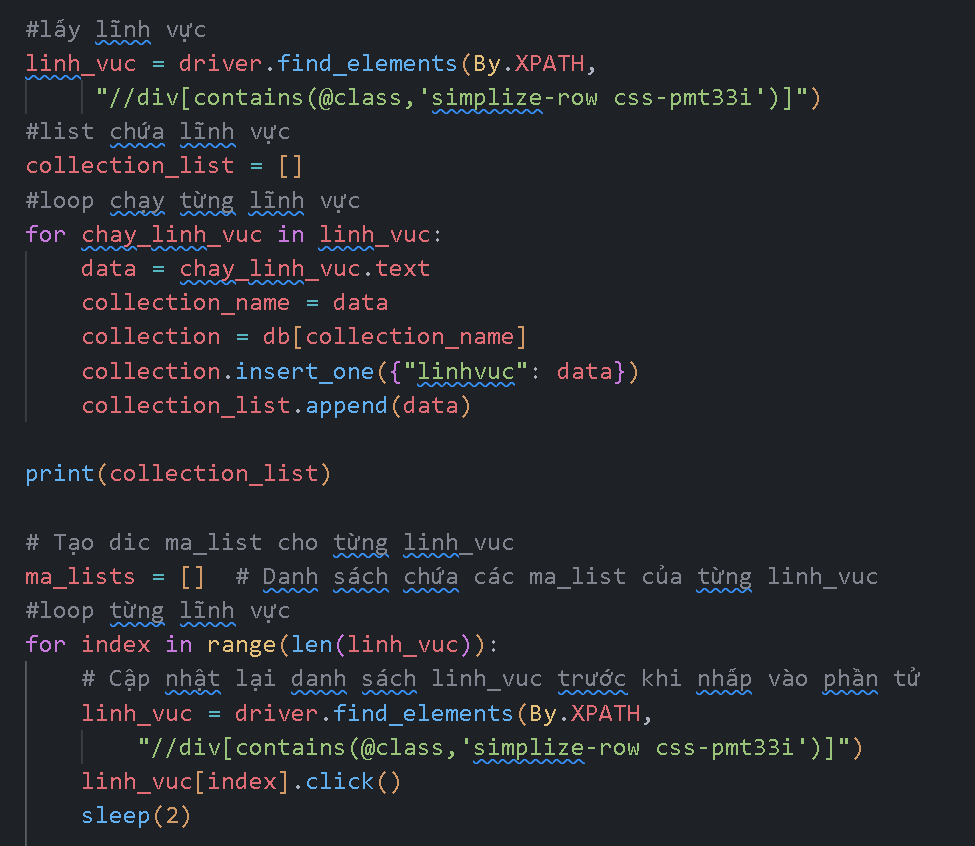
\includegraphics[width=1.0\linewidth]{img/img_chuong3/get_linh_vuc.png}
            \caption{Đoạn mã dùng để truy xuất và thu thập từng lĩnh vực}
            \label{fig:get_linh_vuc}
        \end{figure}
    \end{enumerate}
    
    \subsubsection{\hspace{0.5cm}Truy xuất link từng mã trong từng lĩnh vực cụ thể}

    \begin{enumerate}
        \item []\hspace*{0.7cm}Sau khi lấy được các thông tin các lĩnh vực và thêm các lĩnh vực đó làm collection, sau đó truy cập vào từng lĩnh vực và thu thập danh sách mã từ trang web tương ứng với các lĩnh vực bằng cách tìm các phần tử chứa mã, sau đó thêm chúng vào danh sách \textbf{ma\_list}. Mỗi danh sách mã được in ra và lưu vào danh sách lớn \textbf{ma\_lists}. Sau khi thu thập xong, mã quay lại trang trước để tiếp tục lấy dữ liệu cho lĩnh vực tiếp theo.
    \end{enumerate}
    \begin{enumerate}
        \item[] 
        \begin{figure}[h]
            \centering
            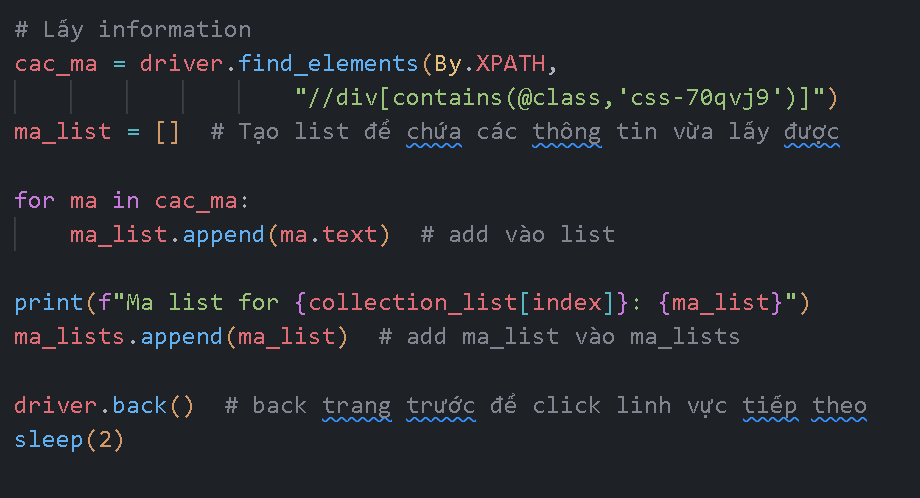
\includegraphics[width=1.0\linewidth]{img/img_chuong3/save_ma_ck.png}
            \caption{Đoạn mã dùng để lưu thông tin danh sách mã chứng khoán.}
        \label{fig:save_ma_ck}
        \end{figure}
    \end{enumerate}
    
    \subsubsection{\hspace{0.5cm}Thu thập dữ liệu lịch sử giá của các mã}
        \begin{enumerate}
            \item []\hspace*{0.7cm}Sau khi thu thập danh sách mã cổ phiếu, đoạn mã tiếp tục duyệt qua từng danh sách mã cổ phiếu trong \textbf{ma\_lists}, sau đó tạo URL tương ứng cho mỗi mã cổ phiếu để truy cập vào trang lịch sử giá. Sau khi trang được tải, mã thực hiện cuộn xuống để đảm bảo toàn bộ dữ liệu đã được tải. Tiếp theo, dữ liệu giá cổ phiếu như ngày, giá mở cửa, giá cao nhất, giá thấp nhất, giá đóng cửa, thay đổi giá, phần trăm thay đổi và khối lượng giao dịch được thu thập từ các hàng trong bảng hiển thị trên trang và lưu vào danh sách \textbf{ls\_gia\_list}. Sau khi thu thập dữ liệu từ một trang, mã tự động nhấn nút "next" để chuyển sang trang tiếp theo, tiếp tục thu thập thêm dữ liệu. Nếu gặp lỗi hoặc không tìm thấy nút chuyển trang, quá trình sẽ dừng lại. Nhờ đó, đoạn mã tự động hóa việc lấy dữ liệu lịch sử giá của nhiều mã cổ phiếu để phục vụ cho phân tích sau này.
        \end{enumerate}
        \begin{enumerate}
            \item[] 
        \begin{figure}[h]
            \centering
            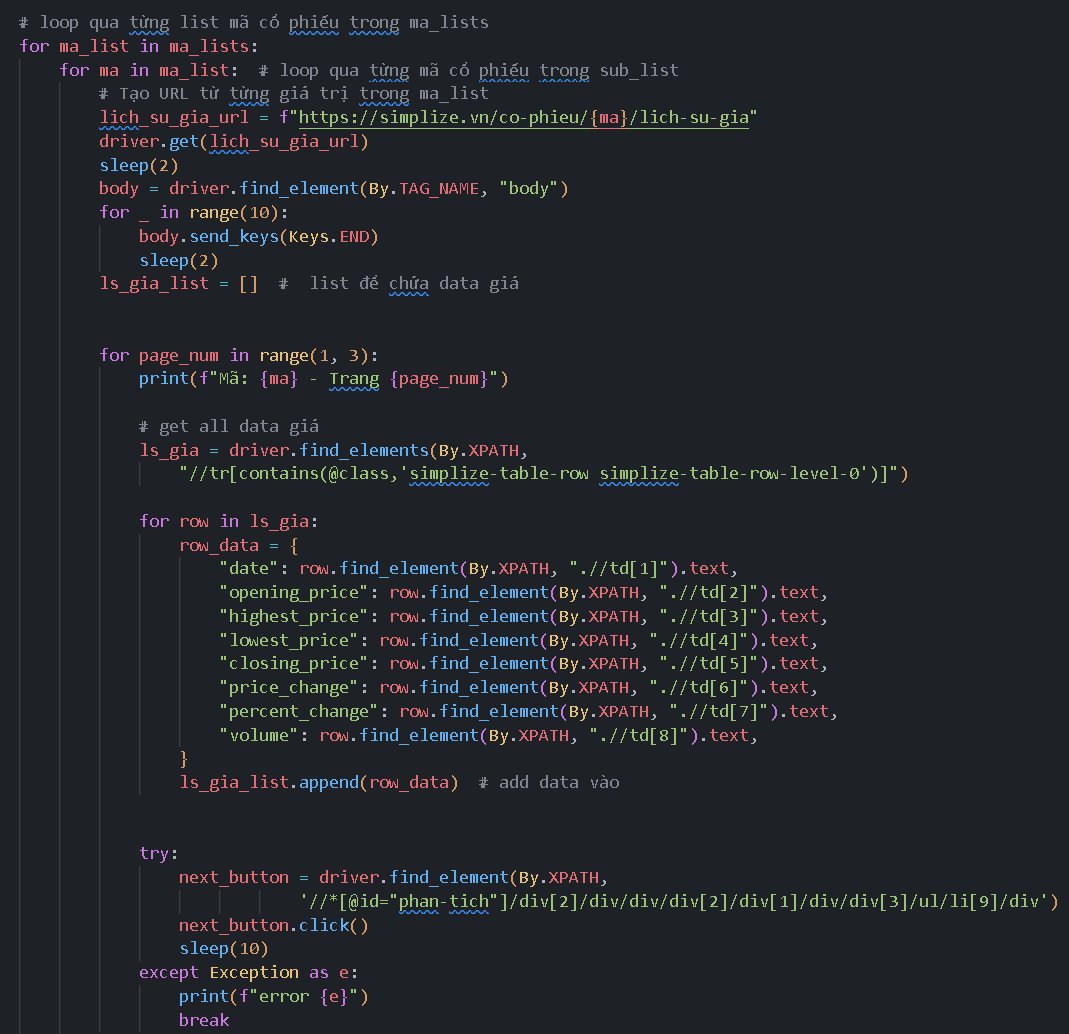
\includegraphics[width=1.0\linewidth]{img/img_chuong3/get_history_price.png}
            \caption{Đoạn mã dùng để thu thập thông tin lịch sử giá của các mã.}
            \label{fig:get_history_price}
        \end{figure}
        \end{enumerate}
\subsubsection{\hspace{0.5cm}Lưu dữ liệu lịch sử giá vào JSON}
\begin{enumerate}
            \item []\hspace*{0.7cm}Sau khi lấy lịch sử giá của các mã thì tiếp tục lưu trữ danh sách dữ liệu lịch sử giá cổ phiếu vào một tệp JSON và quay lại trang trước để tiếp tục thu thập dữ liệu cho mã cổ phiếu tiếp theo. Cụ thể, sau khi thu thập đủ dữ liệu lịch sử giá từ các trang, danh sách \textbf{ls\_gia\_list} sẽ được lưu vào một tệp JSON với tên định dạng \textbf{{ma}\_lich\_su\_gia.json}, trong đó \textbf{ma} là mã cổ phiếu tương ứng. Sau khi lưu dữ liệu thành công, lệnh \textbf{driver.back()} được thực hiện để quay lại trang trước và tiếp tục quá trình thu thập dữ liệu cho mã cổ phiếu tiếp theo trong danh sách. 
        \end{enumerate}
        \begin{enumerate}
            \item[] 
        \begin{figure}[h]
            \centering
            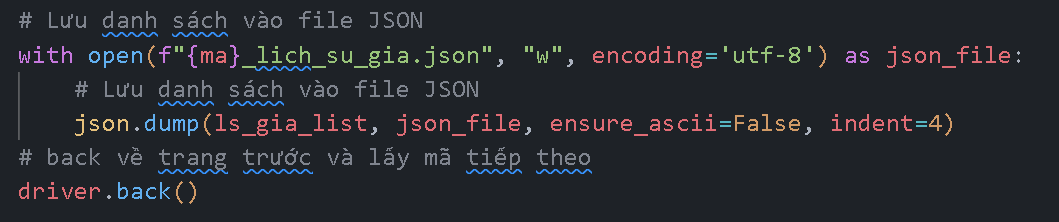
\includegraphics[width=1.0\linewidth]{img/img_chuong3/save_data_json.png}
            \caption{Đoạn mã dùng lưu dữ liệu lịch sử giá của mã vào file JSON}
            \label{fig:save_data_json}
        \end{figure}
        \end{enumerate}
\subsubsection{\hspace{0.5cm}Thu thập dữ liệu hồ sơ doanh nghiệp của các mã}
\begin{enumerate}
            \item []\hspace*{0.7cm}Cũng tương tự cách lấy lịch sử giá thì đoạn mã này dùng để thu thập thông tin hồ sơ doanh nghiệp cho từng mã cổ phiếu và lưu trữ chúng vào file JSON. Đầu tiên, mã khởi tạo một danh sách rỗng \textbf{ho\_so\_data\_list} để chứa dữ liệu. Sau đó, nó lặp qua từng danh sách mã cổ phiếu trong \textbf{ma\_lists} và tạo URL cho hồ sơ doanh nghiệp dựa trên mã cổ phiếu. Tiếp theo, mã tìm kiếm các phần tử chứa thông tin hồ sơ doanh nghiệp bằng cách sử dụng \textbf{find\_elements} với XPath tương ứng. Dữ liệu được lưu vào danh sách \textbf{ho\_so\_list} bằng cách lặp qua các phần tử và thêm vào danh sách. Cuối cùng, danh sách \textbf{ho\_so\_list} được lưu vào file JSON với tên định dạng \textbf{{ma}\_ho\_so\_doanh\_nghiep.json}, trong đó \textbf{ma} là mã cổ phiếu tương ứng. Nhờ đó, tự động hóa quy trình thu thập và lưu trữ thông tin hồ sơ doanh nghiệp cho nhiều mã cổ phiếu khác nhau. 
        \end{enumerate}
        \begin{enumerate}
            \item[] 
        \begin{figure}[h]
            \centering
            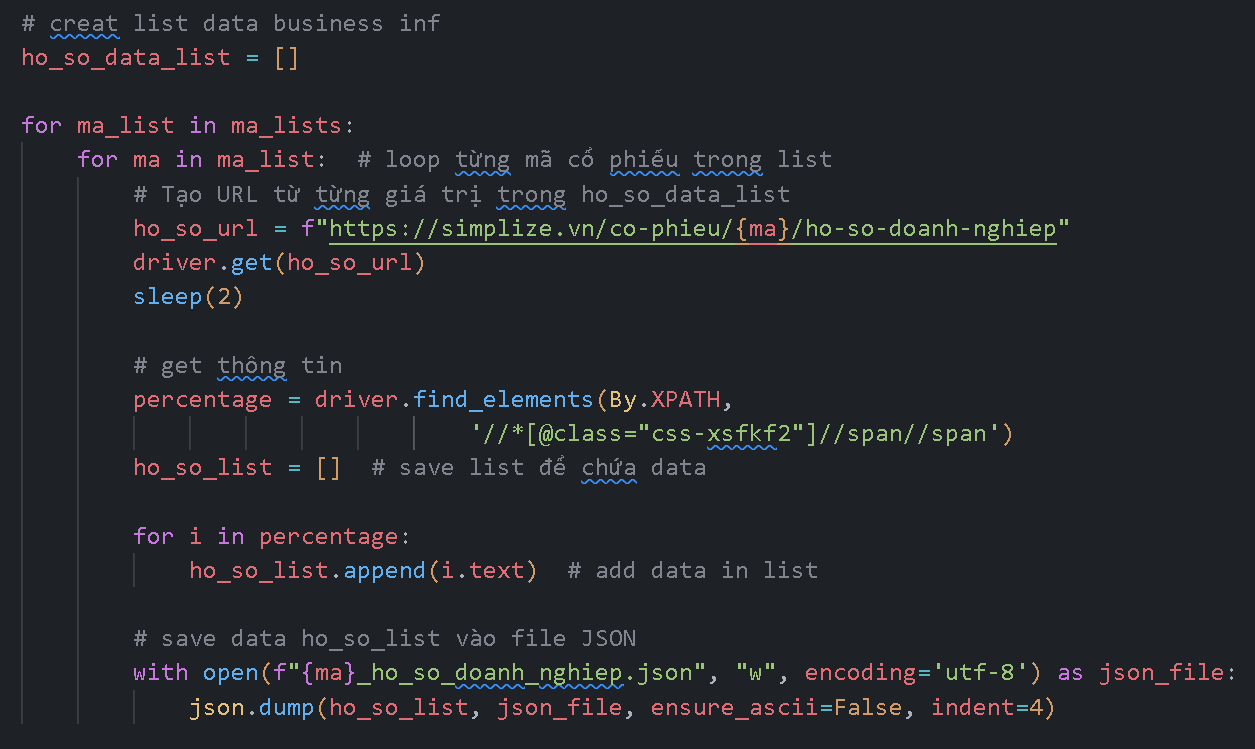
\includegraphics[width=0.9\linewidth]{img/img_chuong3/get_business_inf.png}
            \caption{Đoạn mã dùng để lấy dữ liệu hồ sơ doanh ngiệp của các mã và lưu vào JSON.}
            \label{fig:get_business_inf}
        \end{figure}
        \end{enumerate}

\subsubsection{\hspace{0.5cm}Cập nhật dữ liệu lịch sử giá và hồ sơ doanh nghiệp cho từng mã}
\begin{enumerate}
            \item []\hspace*{0.7cm}Cuối cùng đoạn mà dùng để thực hiện việc cập nhật dữ liệu lịch sử giá và hồ sơ doanh nghiệp cho từng mã cổ phiếu trong các collection. Đầu tiên, mã lặp qua từng danh sách mã cổ phiếu trong \textbf{ma\_lists} và xác định tên lĩnh vực tương ứng từ \textbf{collection\_list}, sau đó truy cập vào collection này. Tiếp theo, mã kiểm tra sự tồn tại của các file JSON chứa dữ liệu lịch sử giá \textbf{(lich\_su\_gia.json)} và hồ sơ doanh nghiệp \textbf{(ho\_so\_doanh\_nghiep.json)}. Nếu các file này tồn tại, dữ liệu sẽ được tải vào các biến tương ứng là \textbf{ls\_gia\_list} và \textbf{ho\_so\_list}. Cuối cùng, đoạn mã sử dụng phương thức \textbf{update\_one} để cập nhật thông tin trong collection với các trường mới cho lịch sử giá và hồ sơ doanh nghiệp của từng mã cổ phiếu.
        \end{enumerate}
        \begin{enumerate}
            \item[] 
        \begin{figure}[h]
            \centering
            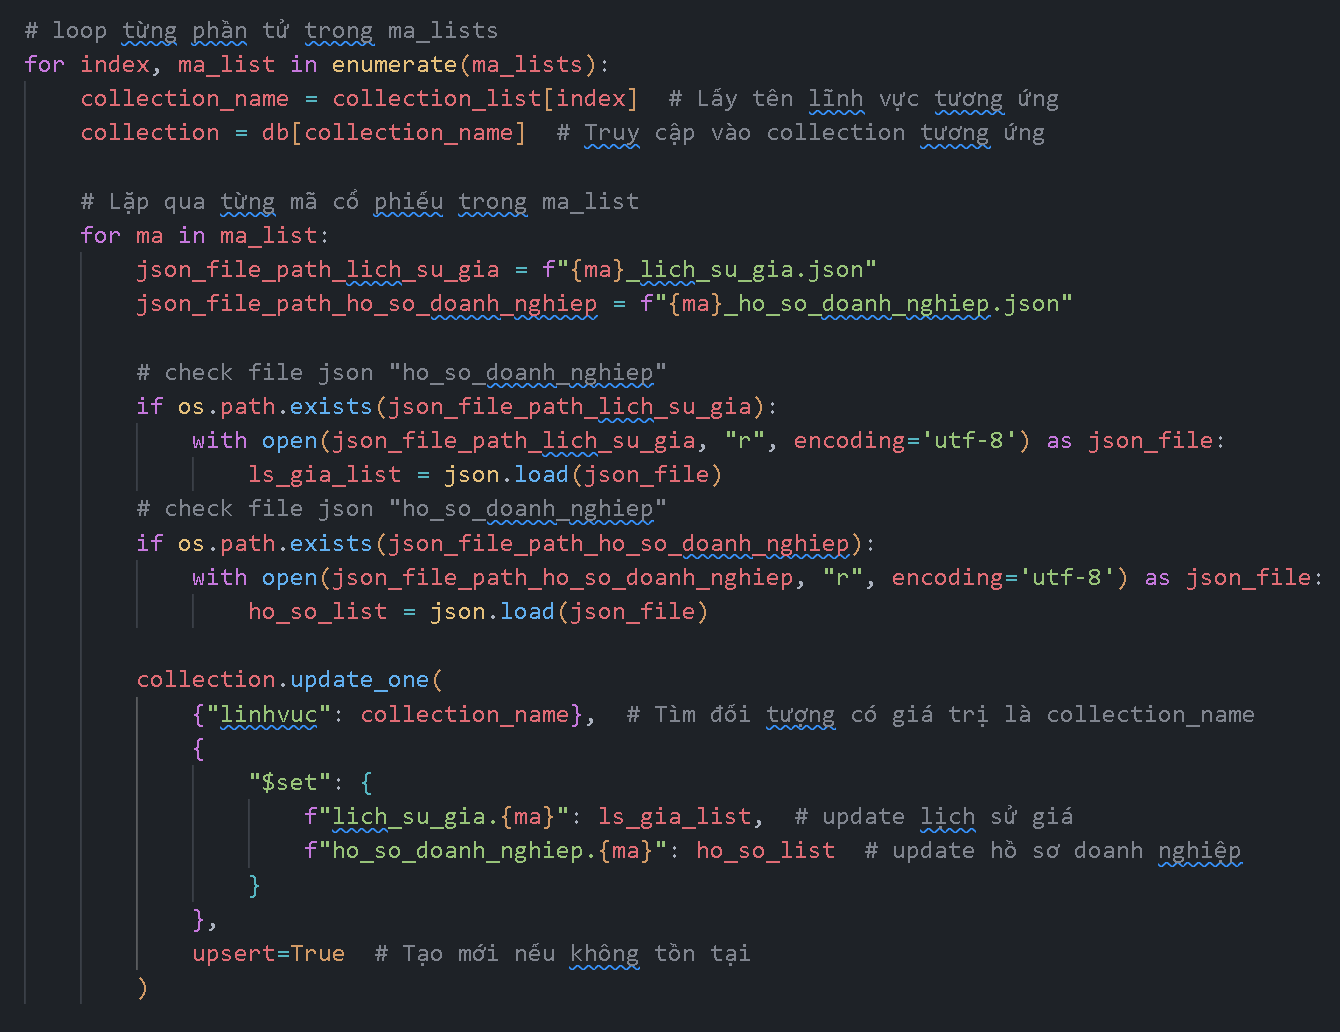
\includegraphics[width=1.0\linewidth]{img/img_chuong3/update_data.png}
            \caption{Đoạn mã dùng để cập nhật dữ liệu cho các mã.}
            \label{fig:update_data}
        \end{figure}
        \end{enumerate}

\subsection{Lưu trữ dữ liệu với MongoDB}
\begin{enumerate}
    \item[] \hspace*{0.7cm}Sau khi đã hoàn thành việc thu thập dữ liệu, chúng tôi sử dụng \\MongoDB để lưu trữ cũng như truy vấn dữ liệu cho tương lai, mỗi mã chứng khoán sẽ được lưu vào các collection tương ứng trong cơ sở dữ liệu.
    \item[] \hspace*{0.7cm}Khi hoàn tất thu thập thì thực hiện đóng kết nối với MongoDB:
    \begin{center}
        \textbf{client.close()}
    \end{center}
\end{enumerate}
\begin{enumerate}
    \item []
    \item []
\end{enumerate}
\section{Mô tả dữ liệu}

\begin{enumerate}
    \item []\hspace{0.7cm}Dữ liệu thu thập được từ trang web simplize.vn gồm lịch sử giá của các mã chứng khoán, cổ phiếu. Với các thuộc tính sau:
    
    \begin{table}[h!]
    \begin{tabular}{|>{\centering\arraybackslash}p{3.8cm}|>{\centering\arraybackslash}p{5.5cm}|>{\centering\arraybackslash}p{5.5cm}|}
    \hline
    \textbf{Tên biến} & \textbf{Mô tả} & \textbf{Kiểu dữ liệu} \\ \hline
    %dòng 1
    Ngày & Ngày ghi nhận giao dịch & Date\\ \hline
    %dòng 2
    Giá mở cửa & Giá đầu tiên trong phiên giao dịch	 & Float\\ \hline
    %dòng 3
    Giá cao nhất & Giá cao nhất trong phiên giao dịch & Float\\ \hline
    %dòng 4
    Giá thấp nhất  & Giá thấp nhất trong phiên giao dịch & Float \\ \hline
    %dòng 5
    Giá đóng cửa & Giá cuối cùng trong phiên giao dịch & Float\\ \hline
    %dòng 6
    Thay đổi giá & Sự thay đổi của giá đóng cửa so với ngày trước & Integer \\ \hline
    %dòng 7
    \% Thay đổi & Tỷ lệ phần trăm thay đổi so với ngày trước & Float \\ \hline
    %dòng 8
    Khối lượng & Số lượng cổ phiếu giao dịch& Integer\\ \hline
    
    \end{tabular}
    \caption{Bảng mô tả các biến và kiểu dữ liệu của chúng.}
    \label{tab:data_type}
    \end{table}
    
\end{enumerate}
\newpage
\section{Sơ đổ quá trình thu thập dữ liệu}
\begin{enumerate}
    \item []
    \item[] 
    \begin{figure}[h]
        \centering
        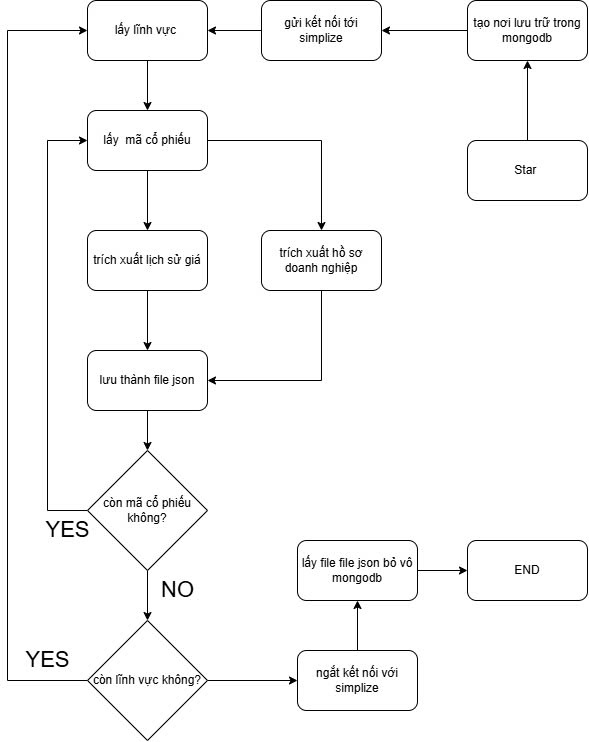
\includegraphics[width=0.8\linewidth]{img/img_chuong3/sodoquatrinh.jpg}
        \caption{Sơ đồ quá trình thu thập và xử lý dữ liệu}
        \label{fig:scraping and processing data}
    \end{figure}
    
\end{enumerate}